\documentclass[preprint]{aastex}

\usepackage{float}
\bibliographystyle{apj}

\begin{document}

\title{The dimensionality of stellar abundance space using red clump stars from APOGEE}
\author{Natalie Price-Jones, supervised by Professor Jo Bovy}

\begin{abstract}
Recent spectroscopic surveys have provided abundant data on stars in the Milky Way. I analyze a subset of data from the Apache Point Observatory Galactic Evolution Experiment (APOGEE) survey, in the form of red clump stars. These metal-enriched stars offer a complex abundance space to explore, which I will do by studying the spectra themselves, rather than derived abundances. This direct use of the spectra facilitates the characterization of errors and systematic effects in interpretation of absorption features. An understanding of these uncertainties allows accurate investigation of the multi-dimensional abundance space, which may reveal trends in abundances with stellar age and position throughout the Milky Way, offering the potential for chemical tagging. Tracing out a star's abundances and these possible trends offers a way to investigate the dynamical and formation history of the Milky Way.

%These trends may also provide a comparative method to assess uncertainties associated with current abundance calculations.
\end{abstract}

\section{Introduction}
\label{sec:back}

A star's history, from its formation environment to its migratory motions, can be traced through its composition. Measuring elemental abundances from stellar spectra establishes this composition. However, current methods for calculating these abundances require robust theoretical models and complete understanding of measurement uncertainties. At present, these methods still exhibit systematic trends with other stellar properties, such as effective temperature $T_{\rm eff}$ or surface gravity $\log(g)$ \citep{holtzman2015}. Removing these contaminating effects from abundance calculations entirely may reveal statistically significant correlations between abundances and stellar age or location within a galaxy. With sufficiently high accuracy in abundance measurements, it may become possible to perform chemical tagging, identifying clusters in abundance data as groups of stars that formed from the same gas cloud but are now dispersed throughout the Galaxy \citep{newgalaxy}. However, 

% any other specific surveys to mention
Recent large-volume spectroscopic survey data from the Apache Point Observatory Galactic Evolution Experiment (APOGEE, \citealt{APOGEE}), upcoming data from Gaia \citep{GAIA} and Galactic Archaeology with HERMES \citep{galah} will offer rich spectral information about hundreds of thousands of stars. The quantity of stars provides a well populated abundance space. To take advantage of this, I develop an efficient method for determining important dimensions of abundance space based on the work of \citealt{openclusters}. The method, described in \S\ref{sec:methods}, uses spectra directly, rather than quantities derived by fitting multi-parameter model spectra. This reduces complexity in calculations of uncertainty, and is less sensitive to the systematic effects of other stellar properties than traditional model fitting methods. Thus I perform a more accurate investigation the dimensionality of abundance space for a sample of stars, including probing the relative significance of particular elements. I apply this method to red clump star spectra from APOGEE, while using open cluster stars with low abundance space scatter as a calibration sample . An understanding of trends in this space may place constraints on what chemical processes contributed to the formation of populations of stars, and clusters of stars in abundance space may correspond to co-natal groups. Identifying these groups through chemical tagging and understand formation processes may reveal details of the Milky Way's star formation history and statistically trace how stars moved through the Milky Way after their formation.


\section{Data Set}
\label{sec:data}
This work analyzes the spectra of a sample of red clump stars from APOGEE's Data Release 12. These stars are selected as belonging to the red clump according to cuts in gravity, effective temperature, and metallicity, and leave us with an initial sample of 19936 stars \citep{bovy2014}. A sample of stars from open clusters is used for calibration \citep{openclusters}. The stars trace, to some extent, the stellar population of the Milky Way through the volume of the APOGEE survey, which covers a significant fraction of the Milky Way’s disk. Data comes in the form of infrared (H-band) spectra covering a wavelength range from 1.514 $\mu$m to 1.696 $\mu$m (with some small nm gaps between detectors) with 7214 pixels \cite{APOGEE}). APOGEE's DR12 pipeline \citep{ASPCAP} provides data on effective temperature ($T_{\rm eff}$), surface gravity ($\log g$), overall metallicity ($Z$), and alpha-element enhancements ([$\alpha$/Fe]), as well as abundances of 15 elements: C, N, O, Na, Mg, Al, Si, S, K, Ca, Ti, V, Mn, Fe, Ni \citep{holtzman2015}. I analyze all 15 of these elements by calculating their abundances directly from spectra.

\section{Methods}
\label{sec:methods}

 %Talk about how open clusters are used for calibration
 
Starting with a sample of APOGEE spectra, I perform empirical fits to remove non-abundance stellar properties. I use spectra processed by the pipeline used to generate stellar parameters and chemical abundances, (ASPCAP - \citealt{ASPCAP}). These spectra are the combined results of all APOGEE spectra taken for a particular star. I begin by masking pixels in the spectra using the bitmask provided by the pipeline. Bits set in the bitmask indicate particular problems with individual pixels in that spectrum, including flags for the effects of cosmic rays, pixel saturation, atmospheric absorption, poor quality calibration files or inaccurate flux uncertainty estimations. I mask on all of the effects listed as well as on pixels with a signal to noise ratio (SNR) below 50.  The result is a masked set of spectra, and a set of associated measurement uncertainties to which the mask on the spectra is applied.

\begin{figure}[H]
\centering
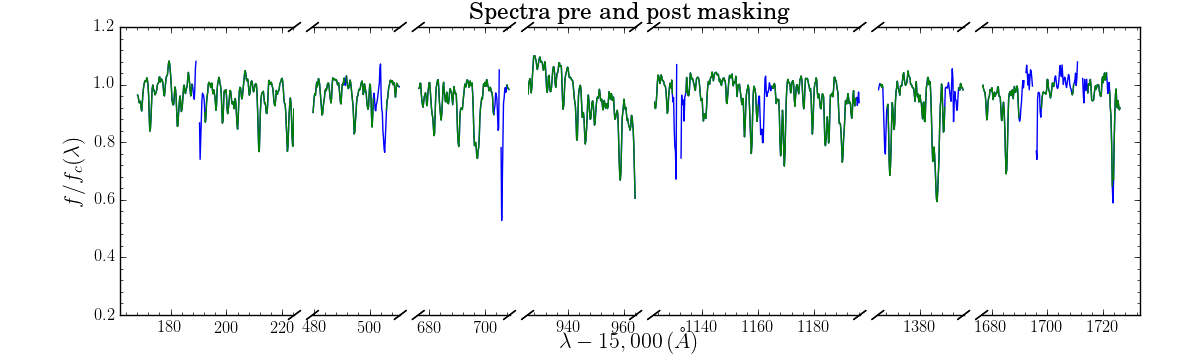
\includegraphics[width = \linewidth]{examplespectrum.png}
\caption{}
\label{fig:spectra}
\end{figure}

After masking the spectra and making corrections to the uncertainties,  the spectra are split into a sample of red clump stars and a calibration sample of open clusters stars. The calibration sample is treated first: the unmasked flux values $(F_p(s))$ at a given pixel $p$  for a star $s$  are weighted by their uncertainties and fit with a second order polynomial in $T_{\rm eff}(s)$. Some function $f_p(s,T_{\rm eff})$ for flux is found  and residuals are calculated from this fit function at each star: $\delta_{p}(s) = F_p(s) - f_p(s,T_{\rm eff})$. The mask of the fitted spectra is then applied to these residuals.

\begin{figure}[H]
\centering
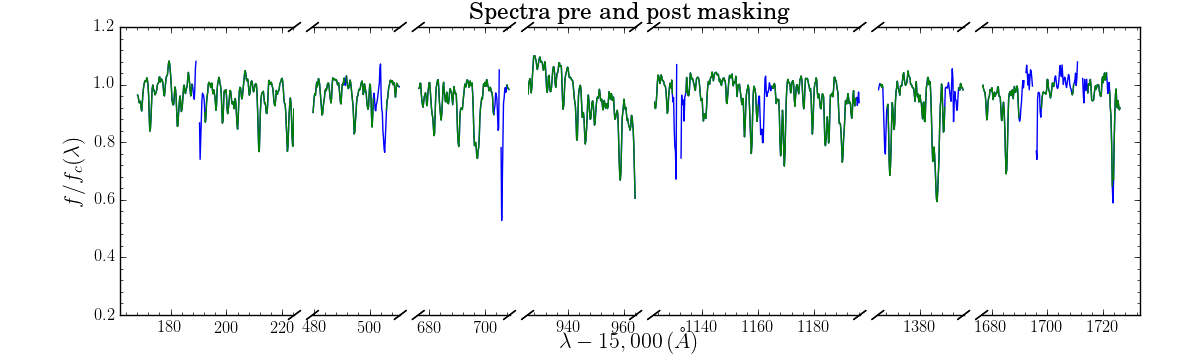
\includegraphics[width = \linewidth]{examplespectrum.png}
\caption{}
\label{fig:spectra}
\end{figure}


Open cluster stars are chemically homogeneous, and so have little scatter in abundance space \citep{openclusters} Any residuals from $f_p(s,T_{\mathrm{eff}})$ represent measurement uncertainty rather than intrinsic variation between pixels. This fact is used to calibrate the red clump sample uncertainties $\sigma_p(s)$. Elements of a covariance matrix $\mathrm{cov}_{p_i,p_j}$ are computed from the array $\delta_p(s)/\sigma_p(s)$ for each star in the open cluster sample. The red clump uncertainties are corrected by the diagonal elements of this covariance matrix: $\sigma_{p,\mathrm{corr}}(s) = \mathrm{cov}_{p,p}\cdot\sigma_{p}(s)$ .  

% say something about splitting the red clump sample for fitting
Using these new corrected uncertainties, the red clump sample is fit in the same way as the open cluster sample way, but with more stellar properties. This results in a second order fit function $f_p(s,T_{\mathrm{eff}},\log g, [\mathrm{Fe/H}])$, where $\log g$ is the surface gravity of the star and [Fe/H] is the iron abundance.

%I then perform a correction on pixels where uncertainties seem underestimated (SNR $>$ 200) increasing the uncertainties calculated by ASPCAP at those pixels until the new SNR does not exceed 200 at any pixel.

% plot example spectrum before and after masking

% be explicit on how fitting works

% plot residuals example

The residuals from the fit comprise the abundance space I proceed to investigate. Trends relating to the bulk properties of the star have been removed by the polynomial fit. Any deviation from the fit that remains must be attributed to differences in stellar abundances. In its raw form, the data $\delta$(p) populates a space in which each pixel is an apparently independent dimension. We can analyze these residuals directly, using expectation maximized principal component analysis (EMPCA - \citealt{empca}).  This algorithm determines which dimensions of a data set represent the most variance, and produces eigenvectors along these dimensions, ranked by how much of the data's variance they explain. Applying EMPCA to the residuals returns eigenvectors with 7214 elements (the number of pixels in the input spectra). Pixels at which these eigenvectors have a large magnitude highlight wavelengths at which stellar flux (i.e. the depth of absorption features) varies the most across the sample. Determining which absorption features are most important for describing variance tells me which elements are best at distinguishing individual stars.

However, individual pixels in a stellar spectra are not uncorrelated and do not represent independent dimensions in abundance space. In particular, pixels at which different absorption features for the same element occur will be correlated with each other. To account for this, and with additional effect of making the data set more easily tractable on a human level, a parallel set of approaches was used to reduce the dimension of abundance space. In one stream, EMPCA was applied directly to the residuals $\delta$. The resulting eigenvectors were weighted according window functions describing absorption features for the 15 elements identified in \S \ref{sec:data}. In an alternate stream, the residuals were first weighted by these window functions, then EMPCA was applied. The results are in A FIGURE.

%Before running PCA with each pixel as an independent dimension we can get a broad sense of the influence of a particular element X by constructing a set of weighted residuals for that element. Residuals for element X pixels are weighted by normalized window functions which trace each X absorption feature and are then summed for each stellar spectrum. Performing PCA on these results reduces the problem from having dimension equal to the number of pixels to having dimensions equal to the number of elements (15). The resulting PCA eigenvectors will show which element (if any) is dominate in determining the residuals after other stellar parameters have been removed.


\section{Timeline}
\label{sec:timeline}

\begin{itemize}
\item Nov 2015, Q: Can I see scatter in residuals of individual elements above our level of intrinsic and measurement uncertainty?
\begin{itemize}
\item Characterize measurement scatter by drawing from a Gaussian determined by the uncertainty in flux measurements. [DONE]
\item Fit open clusters (from \citealt{meszaros2015}) in $T_{\rm eff}$ according to the outline in \S3 and take residuals from this fit as representative of intrinsic abundance scatter. [DONE]
\end{itemize}
\item Dec 2015, Q: What is the dimensionality of abundance space for all elements? Which elements are most significant for distinguishing stars?
\begin{itemize}
\item Use principal component analysis to identify elements of primary importance and the number of dimensions that are not due to noise. [MODIFIED - NOW DOING THIS ON ALL PIXEL SPACE AS WELL - CODE WORKS WITH PRELIMINARY WEIGHT ESTIMATES]
\item Write a code to test existing fitting framework [NEW - DONE]
\item Assess uncertainties from pixel fit. [NEW - CODE EXISTS, NOT YET RUN ON RED CLUMP DATA]
\item Decide on appropriate weights for red clump sample based on results from open clusters. Use open clusters to correct given uncertainties at each pixel [NEW]
\end{itemize}
\item Jan 2016 Q: How can we most accurately find weights for PCA?
\begin{itemize}
\item Trace sources of uncertainty through data (i.e. uncertainty from fitting - how does this translate to uncertainty in open cluster pixel corrections? how in turn does this translate to uncertainty in red clump residuals, which also have uncertainty from their own fitting? this is necessary for accurate weights). [NEW]
\item Use newly more accurate weights in EMPCA in both pixel residual and weighted residual spaces. Use empca.R2(n) where n in the number of the eigenvector to determine where the explained variance is equivalent to the noise variance. How many eigenvectors are needed to explain the variance in each space (pixel vs weighted)? [NEW]
\end{itemize}
\item Feb 2016, Q: Is there any positional dependence of populations in small bins in the remaining dimensions of abundance space?
\begin{itemize} 
\item Collect stars from small bins in the multidimensional residual space and plot their radial and vertical positions.
\item Determine if stars belonging to different bins inhabit different sections of the galaxy, as well as positional variations for stars within a bin.
\end{itemize}
\item Mar/Apr 2016, Q: Can I understand the reasons certain elements may be more significant after PCA by modeling spectra?
\begin{itemize}
\item Create model spectra by varying abundances of the 15 elements.
\item Perform fitting described in \S\ref{sec:methods} and compare with fitting done on APOGEE data. Ascertain whether model spectra created with derived abundances for the red clump stars can reproduce residual results from the data set.
\end{itemize}
\end{itemize}

\bibliography{update}

\end{document}